%%%%%%%%%%%%%%%%%%%%%%%%%%%%%%%%%%%%%%%%%
% Template ini dibuat untuk makalah seminar mahasiswa
% Program Alih Jenis (Ekstensi) Ilmu Komputer IPB
% Version 1.0 (18/05/2015)
%
% Template ini menggunakan template yang di-download dari:
% http://www.LaTeXTemplates.com
% Mathias Legrand (legrand.mathias@gmail.com)
% License: CC BY-NC-SA 3.0 (http://creativecommons.org/licenses/by-nc-sa/3.0/)
%
% Dimodifikasi untuk keperluan Program Studi
% Oleh: JULIO ADISANTOSO (julioipb@gmail.com)
%
% Untuk memudahkan penggunaan, maka diambil contoh makalah atas nama 
% Luthfi Noviandi di bawah bimbingan Julio Adisantoso ILKOM-IPB.
% Silakan mengganti dan melengkapi file:
%    (1) seminar_information.tex -- judul, nama, nim, email, pembimbing, dsb
%    (2) abstrak.tex -- abstrak makalah
%    (3) pendahuluan.tex -- berisi latar belakang, dsb
%    (4) metode.tex -- berisi metode penelitian
%    (5) hasil.tex -- berisi hasil dan pembahasan
%    (6) daftar_pustaka.tex -- berisi daftar pustaka
%
%%%%%%%%%%%%%%%%%%%%%%%%%%%%%%%%%%%%%%%%%

%----------------------------------------------------------------------------------------
%	PACKAGES AND OTHER DOCUMENT CONFIGURATIONS
%----------------------------------------------------------------------------------------

\documentclass[fleqn,11pt]{SelfArx} % Document font size and equations flushed left
\usepackage[english]{babel}

%----------------------------------------------------------------------------------------
%	COLUMNS
%----------------------------------------------------------------------------------------

\setlength{\columnsep}{0.55cm} % Distance between the two columns of text
\setlength{\fboxrule}{0.75pt} % Width of the border around the abstract

%----------------------------------------------------------------------------------------
%	COLORS
%----------------------------------------------------------------------------------------

\definecolor{color1}{RGB}{0,0,90} % Color of the article title and sections
\definecolor{color2}{RGB}{0,20,20} % Color of the boxes behind the abstract and headings

%----------------------------------------------------------------------------------------
%	HYPERLINKS
%----------------------------------------------------------------------------------------

\usepackage{hyperref} % Required for hyperlinks
\hypersetup{hidelinks,colorlinks,breaklinks=true,urlcolor=color2,citecolor=color1,linkcolor=color1,bookmarksopen=false,pdftitle={Title},pdfauthor={Author}}


%
% Hyphenation untuk Indonesia 
%
% @author  Andreas Febrian
% @version 1.00
% 
% Tambahkan cara pemenggalan kata-kata yang salah dipenggal secara otomatis 
% oleh LaTeX. Jika kata tersebut dapat dipenggal dengan benar, maka tidak 
% perlu ditambahkan dalam berkas ini. Tanda pemenggalan kata menggunakan 
% tanda '-'; contoh: menarik  --> pemenggalan: me-na-rik
%

\hyphenation{
    % alphabhet A
    a-na-li-sa a-tur ada-lah
    a-pli-ka-si 
    % alphabhet B
    ba-ngun-an 
    be-be-ra-pa 
    ber-ge-rak
    ber-ke-lan-jut-an 
    ber-pe-nga-ruh ber-no-ul-li
    % alphabhet C
    ca-ri
    % alphabhet D
    di-sim-pan di-pim-pin de-ngan da-e-rah di-ba-ngun da-pat di-nya-ta-kan 
    di-sim-bol-kan di-pi-lih di-li-hat de-fi-ni-si di-kem-bang-kan di-be-ri-kan
    % alphabhet E
    e-ner-gi eks-klu-sif
    % alphabhet F
    fa-si-li-tas
    % alphabhet G
    ga-bung-an ge-rak
    % alphabhet H
    ha-lang-an
    % alphabhet I
    % alphabhet J
    jang-krik
    % alphabhet K
    ke-hi-lang-an
    ku-ning 
    kua-li-tas ka-me-ra ke-mung-kin-an ke-se-pa-ham-an
    % alphabhet L
    ling-kung-an
    % alphabhet M
    me-neng-ah
    meng-a-tas-i me-mung-kin-kan me-nge-na-i me-ngi-rim-kan 
    meng-u-bah meng-a-dap-ta-si me-nya-ta-kan mo-di-fi-ka-si
    meng-a-tur meng-um-pul-kan meng-hi-tam-kan
    % alphabhet N
    nya-ta non-eks-klu-sif
    % alphabhet O
    % alphabhet P
	pe-nye-rap-an 
	pe-ngon-trol
    pe-mo-del-an
    pe-ran  pe-ran-an-nya
    pem-ba-ngun-an pre-si-den pe-me-rin-tah prio-ri-tas peng-am-bil-an 
    peng-ga-bung-an pe-nga-was-an pe-ngem-bang-an 
    pe-nga-ruh pa-ra-lel-is-me per-hi-tung-an per-ma-sa-lah-an 
    pen-ca-ri-an peng-struk-tur-an
    % alphabhet Q
    % alphabhet R
    ran-cang-an 
    ring-kas-an
    % alphabhet S
    si-mu-la-si sa-ngat
    % alphabhet T
    te-ngah
    ter-da-pat
    % alphabhet U
    % alphabhet V
    % alphabhet W
    % alphabhet X
    % alphabhet Y
    % alphabhet Z
    % special
}
% Tuliskan nama lengkap Anda
\def\namaMhs {Bayu Santoso}

% Tuliskan NIM Anda
\def\nim {G64134017}

% Tuliskan alamat email Anda
\def\emailMhs {bayusantoso.mail@gmail.com }

% Tuliskan nama lengkap dosen pembimbing
\def\namaDosen {Yeni Herdiyeni}

% Tuliskan judul seminar di definisi "judul"
\def\judul {Pembangunan \textit{Biodiversity Informatics} Genetika Tumbuhan Berbasis Ontologi}

% Tuliskan judul seminar dalam Bahasa Inggris di definisi "judulen"
\def\judulen {}

% Tuliskan kata kunci, dipisahkan oleh tanda titik-koma
\def\katakunci {\textit{biodiversity informatics}; tumbuhan; ontologi; web semantik}

% Tuliskan kata kunci dalam bahasa Inggris, dipisahkan oleh tanda titik-koma
\def\katakuncien {}

% Tuliskan tanggal pelaksanaan seminar
\def\tglseminar {8 September 2015}
\usepackage{xcolor,colortbl}
\usepackage{multicol}
\usepackage{multirow}
\usepackage[urldate=iso8601, backend=biber, style=authoryear, url=true, doi=true, sorting=nyt]{biblatex}
\addbibresource{pustaka.bib}
\DefineBibliographyStrings{english}{%
	urlseen = {diunduh pada},
}
\renewbibmacro{in:}{\xspace dalam:}
\renewbibmacro*{volume+number+eid}{%
	\printfield{volume}%
	%  \setunit*{\adddot}% DELETED
	\setunit*{\addnbspace}% NEW (optional); there's also \addnbthinspace
	\printfield{number}%
	\setunit{\addcomma\space}%
	\printfield{eid}}
\DeclareFieldFormat[article]{number}{\mkbibparens{#1}}


%----------------------------------------------------------------------------------------
%	ARTICLE INFORMATION
%----------------------------------------------------------------------------------------

\JournalInfo{Makalah Seminar Program S1 Ilmu Komputer Alih Jenis} % Journal information
\Archive{Departemen Ilmu Komputer, FMIPA-IPB\\ \tglseminar} % Departemen ILKOM-IPB

\PaperTitle{\judul\\ \small \textit{\judulen}\normalsize } 

\Authors{\namaMhs (\nim)*, \namaDosen} % Penulis
\affiliation{*\scriptsize\textbf{Email}: \emailMhs \normalsize} % Corresponding author

\Keywords{\scriptsize \katakunci\\ \textit{\katakuncien} \normalsize} 
\newcommand{\keywordname}{Kata Kunci/\textit{Keywords}} % Defines the keywords heading name

%----------------------------------------------------------------------------------------
%	ABSTRACT
%----------------------------------------------------------------------------------------
\Abstract{\scriptsize 
% ---- Tuliskan abstrak di bagian ini seperti contoh.
Indonesia memiliki lebih dari 32.000 spesies tumbuhan. Saat ini hutan Indonesia mengalami kerusakan dan kepunahan. Oleh karena itu, diperlukan upaya untuk melestarikan tumbuhan. Salah satu cara untuk melestarikan tumbuhan adalah dengan cara mengenali spesies tumbuhan tersebut.   Berdasarkan hal tersebut maka muncul bidang baru dalam pengumpulan informasi tumbuhan yang bernama \textit{biodiversity informatics}. Metode pemodelan data yang dapat menangani sistem berbasis inferensi adalah ontologi. Ontologi dapat diterapkan pada web semantik. Penelitian ini akan mengembangkan sistem web semantik yang memberikan informasi genetika tumbuhan. Selain itu juga merumuskan masalah bagaimana melakukan inferensi pengetahuan dari sistem web semantik gen tumbuhan dengan sistem web semantik yang lain.
% ---- Akhir bagian abstrak
\normalsize}


%----------------------------------------------------------------------------------------

\begin{document}

\flushbottom % Makes all text pages the same height

\maketitle % Print the title and abstract box

\thispagestyle{empty} % Removes page numbering from the first page

%----------------------------------------------------------------------------------------
%	BAGIAN PENDAHULUAN
%----------------------------------------------------------------------------------------

%----------------------------------------------------------------------------------------
%	PENDAHULUAN
%----------------------------------------------------------------------------------------
\section*{PENDAHULUAN} % Sub Judul PENDAHULUAN
% Tuliskan isi Pendahuluan di bagian bawah ini. 
% Jika ingin menambahkan Sub-Sub Judul lainnya, silakan melihat contoh yang ada.
% Sub-sub Judul 
\subsection*{Latar Belakang}
Indonesia memiliki lebih dari 32.000 spesies tumbuhan (\citeauthor{BAPPENAS2003} \cite*{BAPPENAS2003}). Saat ini hutan Indonesia mengalami kerusakan dan kepunahan (\citeauthor{ZUHUD2008} \cite*{ZUHUD2008}). Oleh karena itu, diperlukan upaya untuk melestarikan tumbuhan. Salah satu cara untuk melestarikan tumbuhan adalah dengan cara mengenali tumbuhan tersebut. \textit{Biodiversity Informatics} merupakan upaya untuk membuat sumber informasi keanekaragaman hayati global tersedia dalam format digital yang efisien, dan untuk mengembangkan alat yang efektif dalam menganalisis dan memahami data tersebut (\citeauthor{GILLMANE2009} \cite*{GILLMANE2009}). Informasi yang dapat diperoleh dari \textit{biodiversity informatics} adalah informasi mengenai taksonomi, gambar tumbuhan, lingkungan, dan DNA tumbuhan. 

Impementasi dari \textit{biodiversity informatics} sudah menghasilkan beberapa sistem yang menyediakan informasi mengenai tumbuhan.  Integrated Taxonomic Information System  (ITIS) dan Global Biodiversity Information Facility (GBIF) menyediakan informasi yang luas tentang tumbuhan. Proses identifikasi dan pengelolaan informasi keanekaragaman hayati tersebut memerlukan sistem yang terpadu dan holistic dengan menggunakan IPTEKS komputer yang berkembang pesat saat ini (\citeauthor{HERDIYENI2013} \cite*{HERDIYENI2013}). Upaya pemanfaatan IPTEKS yang telah dilakukan seperti diantaranya pembangunan sistem IPB Biodiversity Informatics (IPBiotics) untuk pengelolaan informasi keanekaragaman hayati sumber daya alam Indonesia. Sistem BI tersebut berguna meningkatkan pengelolaan pengetahuan (knowledge management), eksplorasi, analisis, sintesis dan interpretasi data keanekaragaman hayati mulai dari level genomik, level spesies sampai dengan level ekosistem (\citeauthor{HERDIYENI2013} \cite*{HERDIYENI2013}). Pada pengembangan selanjutnya, sistem IPBiotics didesain agar dapat melakukan inferensi pengetahuan. Sistem yang ada saat ini masih menggunakan model basis data relasional. Permasalahannya adalah model basis data relasional kurang sesuai diterapkan pada sistem berbasis inferensi (\citeauthor{LAALLAM2013} \cite*{LAALLAM2013}).  

Ontologi adalah metode yang digunakan untuk merepresentasikan ide, fakta dan lain sebagainya, yang digunakan untuk mendefinisikan hubungan dan klasifikasi dari pengetahuan tertentu (\citeauthor{JEPSEN2010} \cite*{JEPSEN2010}). Ontologi dapat menentukan kelas, hubungan, fungsi dan objek lain (\citeauthor{DILECCE2008} \cite*{DILECCE2008}). Selain itu, model ontologi lebih sesuai diterapkan pada web semantik dibandingkan dengan model basis data relasional (\citeauthor{LAALLAM2013} \cite*{LAALLAM2013}).

Penelitian dengan menggunakan ontologi mengenai tumbuhan sudah banyak dilakukan, seperti penelitian tentang ontologi yang digunakan untuk menganalisis hubungan tumbuhan obat dengan istilah medis yang standar (\citeauthor{VADIVU2012} \cite*{VADIVU2012}). Penelitian yang terkait dengan ontologi gen juga sudah pernah dilakukan untuk menghasilkan data gen yang dinamis dan terkontrol (\citeauthor{ASHBURNERM2000} \cite*{ASHBURNERM2000}) dan pemodelan ontologi tumbuhan obat menggunakan pengetahuan etnobotani (Sanjaya 2014). Namun penelitian tersebut berfokus pada pemodelan ontologi. Berdasarkan latar belakang di atas penelitian ini akan membangun sistem web semantik yang memanfaatkan ontologi yang sudah ada untuk mengelola informasi tumbuhan.

% Sub-sub Judul 
\subsection*{Tujuan}
Tujuan yang ingin dicapai dalam penelitian ini adalah:
\begin{enumerate}[noitemsep] 
\item Membangun sistem \textit{biodiversity informatics} tumbuhan menggunakan ontologi gen (\textit{gene ontology}).
\item Menerapkan sistem inferensi pengetahuan pada ontologi gen untuk mengembalikan informasi berupa \textit{molecular function}, \textit{biological processes} dan \textit{cellular components} yang terdapat pada tumbuhan.
\end{enumerate}

\subsection*{Ruang Lingkup}
Ruang lingkup penelitian adalah:
\begin{enumerate}[noitemsep] 
\item Ontologi yang digunakan dalam penelitian ini berasal dari situs geneontology.org.
\item Membangun \textit{biodiversity informatics} pada level genetik.
\end{enumerate}

\subsection*{Manfaat}
Manfaat yang diinginkan dari penelitian ini adalah membantu proses dokumentasi data dan pengetahuan keanekaragaman hayati tumbuhan. Dengan memanfaatkan ontologi, memungkinkan sistem untuk melakukan inferensi dan mengembalikan informasi detail tumbuhan mengenai \textit{molecular function}, \textit{biological processes} dan \textit{cellular components} tumbuhan. Dengan informasi tersebut, diharapkan proses dokumentasi keanekaragaman hayati tumbuhan berjalan lebih efektif.


%----------------------------------------------------------------------------------------
%	Tinjauan Pustaka
%----------------------------------------------------------------------------------------

%----------------------------------------------------------------------------------------
%	METODE
%----------------------------------------------------------------------------------------
\section*{TINJAUAN PUSTAKA}

\subsection*{\textit{Biodiversity Information}}

\textit{Biodiversity} atau keanekaragaman hayati mengacu pada upaya untuk mempelajari kehidupan di bumi. Keanekaragaman yang dipelajari meliputi bidang molekul, organisme dan ekologi. \textit{Biodiversity information} (BI) merupakan upaya untuk membuat sumber informasi keanekaragaman hayati global tersedia dalam format digital yang efisien, dan untuk mengembangkan alat yang efektif dalam menganalisis dan memahami data tersebut (\citeauthor{GILLMANE2009} \cite*{GILLMANE2009}).  Salah satu tantangan utama dalam BI adalah untuk memberikan data pengetahuan mengenai keanekaragaman hayati dengan cepat, dengan pengetahuan tersebut dapat dibangun sistem keanekaragaman hayati yang terpadu (\citeauthor{GILLMANE2009} \cite*{GILLMANE2009}).

\subsection*{Ontologi}

Ontologi adalah suatu metode yang digunakan untuk merepresentasikan pengetahuan yang mendefinisikan hubungan dan klasifikasi dari pengetahuan tertentu (\citeauthor{JEPSEN2010} \cite*{JEPSEN2010}). Seperti pemrograman berorientasi objek, ontologi juga menggunakan kelas dan \textit{instance} dalam merepresentasikan pengetahuan. Namun, ontologi dengan pemrograman berorientasi objek berbeda dalam implementasinya. Pada pemrograman berorientasi objek \textit{instance} merupakan contoh nyata dari kelas tersebut. Pada ontologi, \textit{instance} bermakna anggota suatu domain tertentu (\citeauthor{JEPSEN2010} \cite*{JEPSEN2010}).

\subsection*{\textit{Gene Ontology} (GO)}

\textit{Gene ontology} (GO) dikembangkan oleh Gene Ontology Consortium untuk memberikan informasi mengenai gen yang lebih dinamis, terkontrol dan memiliki aturan yang sama. Dibuat dari tahun 1998 GO pada awalnya mengkolaborasikan tiga buah \textit{database} organisme yaitu Fly Base (Drosophila), Saccharomyces Genome Database (SGD) dan Mouse Genome Database (MGD). Semenjak itu GO terus berkembang dengan bergabungknya penelitian-penelitian mengenai ontologi gen dari lembaga lain. Saat ini GO sudah menampung data-data mengenai gen tumbuhan, hewan dan mikroba. 

GO memiliki tiga komponen ontology yaitu \textit{Molecular Function}, \textit{Biological Processes} dan \textit{Cellular Components} (\citeauthor{ASHBURNERM2000} \cite*{ASHBURNERM2000}). \textit{Molecular Function} merupakan aktivitas yang terjadi pada level molekular seperti aktivitas katalis atau aktivitas binding.  \textit{Biological processes}  menggambarkan serangkaian kegiatan dengan tujuan tertentu yang melibatkan proses molecular function. \textit{Cellular components} menggambarkan komponen-komponen sel yang merupakan bagian dari objek yang lebih besar sebagai contoh retikulum endoplasma atau nukleus. Selain itu \textit{cellular components} juga memberikan informasi \textit{gene-product}, sebagai contoh \textit{ribosome} dan \textit{proteasome}. Gambar \ref{fig:gene_ontology} merupakan sebagian kecil dari term yang ada di bawah \textit{biological processes}.

\begin{figure}[h!] % Gunakan \begin{figure*} untuk memasukkan Gambar
	\centering
	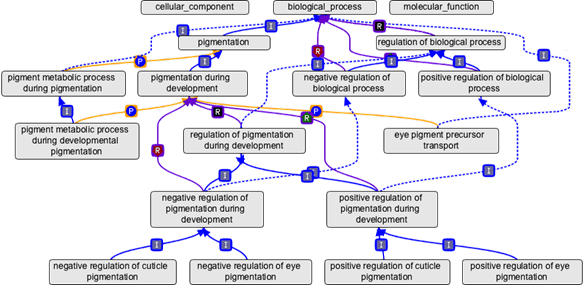
\includegraphics[width=240pt]{geneontology.png}
	\caption{\textit{Term} di bawah \textit{biological processes}}
	\label{fig:gene_ontology}
\end{figure}

\subsection*{\textit{Resource Description Framework} (RDF)}

eXtensible Markup Language (XML) adalah suatu bahasa yang direpresentasikan dengan \textit{metadata}. XML merepresentasikan informasi agar dapat dengan mudah diakses oleh mesin. XML tidak menyediakan tag-tag tertentu, tetapi penggunanya dapat mendefiniskan tag secara mandiri. Namun, XML tidak dapat menunjukkan arti dari suatu data. RDF merupakan suatu bentuk dari data model. RDF mengadopsi sintaks-sintaks yang dimiliki oleh XML. Menurut Antoniou dan Hermalen (\cite*{ANTONIOUG2008}), RDF memiliki konsep dasar RDF yaitu \textit{resource}, \textit{properties}, dan \textit{statement}. \textit{Resource} adalah objek atau tentang sesuatu yang ingin diungkapkan. Beberapa contoh \textit{resource} seperti judul buku, pengarang, penerbit, orang dan sebagainya. Setiap \textit{resource} memiliki \textit{Universal Resource
Identifier} (URI). \textit{Properties} adalah deskripsi hubungan antar \textit{resource}, misalnya properti yang menghubungkan antara buku dengan penulisnya adalah “ditulis oleh”. \textit{Statement} adalah bentuk literal dari \textit{resource}, \textit{properties} dan nilainya. Menurut Raimbault (\cite*{RAIMBAULT2010})), statement disebut juga dengan triple model.

\begin{figure}[h!] % Gunakan \begin{figure*} untuk memasukkan Gambar
	\centering
	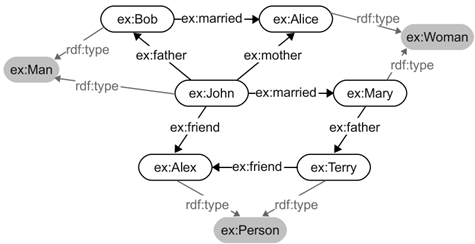
\includegraphics[width=200pt]{model_rdf_contoh_gb1.png}
	\caption{Contoh Model RDF}
	\label{fig:model_rdf}
\end{figure}

Gambar \ref{fig:model_rdf} menunjukkan contoh model RDF yang direpresentasikan dalam bentuk \textit{graph}.  Contoh \textit{statement} yang dapat dilihat dari Gambar \ref{fig:model_rdf} adalah John menikah dengan Mary.

\subsection*{\textit{Web Ontology Language} (OWL)}

\textit{Web Ontology Language} (OWL) adalah bahasa yang digunakan untuk membaca dan mendefinisikan kelas dan properti model RDF (\citeauthor{SEGARAB2009} \cite*{SEGARAB2009}). OWL merupakan bahasa yang kompleks. Oleh karena itu, OWL dibagi menjadi tiga sub bahasa berdasarkan tingkat kompleksitasnya, yaitu OWL-Lite, OWL DL dan OWL Full. OWL-Lite merupakan bentuk sub bahasa OWL yang paling sederhana. OWL DL memiliki fitur yang dapat digunakan untuk memaksimalkan penggunaan sistem \textit{reasoning} dan dapat menjamin kelengkapan informasi yang ingin didapat. OWL Full memberikan fitur yang membebaskan dalam mendeskripsikan sintaks RDF, tetapi tidak menjamin kelengkapan informasi yang didapat (He dan An 2011). OWL memiliki struktur data yang terdiri dari \textit{namespace} dan \textit{ontology head}. \textit{Namespace} digunakan untuk mengelompokkan \textit{identifier}. \textit{Ontology head} digunakan untuk mengumpulkan informasi metadata OWL yang digunakan (\citeauthor{HEG2010} \cite*{HEG2010}).

\subsection*{\textit{Simple Protocol and RDF Query Language} (SPARQL)}

\textit{Simple Protocol and RDF Query Language} (SPARQL) adalah bahasa \textit{query} yang digunakan untuk melakukan query data terhadap model RDF. Sama halnya dengan \textit{query} pada SQL, SPARQL juga digunakan untuk melakukan \textit{query} data-data yang diinginkan. Pembedanya, SQL melakukan \textit{query} pada \textit{database} yang terdiri dari satu atau beberapa tabel, sedangkan SPARQL melakukan \textit{query} pada data RDF yang berupa triple model (Segaran et al. \citeauthor{SEGARAB2009} \cite*{SEGARAB2009}). Berikut contoh sintaks SPARQL:
\\

PREFIX fb:$<$http://rdf.freebase.com/ns/$>$

SELECT ?who ?film

WHERE \{

?film fb:film.film.directed\_by ?who

?film fb:film.film.starring ?who

\}
\\

\textit{Query} dari SPARQL hampir sama seperti pada bahasa \textit{query} yang lain. Seperti sintaks SELECT, WHERE dan lainnya. Sintaks PREFIX digunakan untuk menyingkat alamat sumber dari data ontologi.

\subsection*{\textit{Semantic Web Object Oriented Design Methodology} (SW-OODM)}

\textit{Object Oriented Design Methodology} (OOMD) adalah metode yang digunakan untuk mengembangkan aplikasi web. Metode ini berguna untuk menangkap kebutuhan pengguna. Dengan adanya metode ini aktfitas pengembangan dapat dikontrol dengan baik (\citeauthor{FAROOQA2010} \cite*{FAROOQA2010}). SW-OODM merupakan metode pengembangan aplikasi web semantik yang merupakan pengembangan dari OOMD. SW-OODM meliputi aktivitas yang berguna untuk memformulasikan dan mendeskripsikan pengetahuan, sehingga aplikasi yang dibuat dapat dimengerti baik oleh mesin maupun oleh manusia (\citeauthor{FAROOQA2010} \cite*{FAROOQA2010}). Aktivitas yang terdapat di metode SW-OODM yaitu meliputi analysis phase dan design phase.Tahapan-tahapan yang berada dalam \textit{analysis phase} dikelompokan ke dalam empat model: \textit{preliminary web-ontology model}, \textit{information model}, \textit{user model}, dan \textit{operation model}. Sedangkan pada design phase dikelompokan menjadi enam unit: \textit{namely}, \textit{building component model}, \textit{building navigation model}, \textit{building operation partitioning model}, \textit{web ontology model} dan \textit{semantic web-page design} (Farooq et al. 2010).



%----------------------------------------------------------------------------------------
%	BAGIAN METODE
%----------------------------------------------------------------------------------------

%----------------------------------------------------------------------------------------
%	METODE
%----------------------------------------------------------------------------------------
\section*{METODE PENELITIAN}

\subsection*{Data Penelitian}

Data yang digunakan pada penelitian ini adalah data ontologi gen yang berasal dari situs geneontology.org.

\subsection*{Tahapan Penelitian}

Tahapan-tahapan yang dilakukan pada penelitian ini mengacu pada metode pengembangan aplikasi SW-OODM. Tahapan pengembangan aplikasi SW-OODM dapat dilihat pada Gambar \ref{fig:tahapan_penelitian}.

\begin{figure}[h!] % Gunakan \begin{figure*} untuk memasukkan Gambar
	\centering
	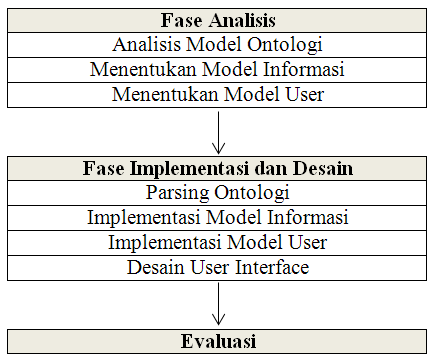
\includegraphics[width=200pt]{kolokium_tahapan_penelitian_gb2.png}
	\caption{Tahapan Penelitian}
	\label{fig:tahapan_penelitian}
\end{figure}

Fase Analisa

Pada fase analisa terdapat 3 aktivitas yang akan dilakukan, yaitu analisis model ontologi, menentukan model informasi, menentukan model user. Aktivitas analisis model ontologi akan diidentifikasi domain yang terdapat pada ontologi gen. Hasil identifikasi model ontologi digambarkan dengan bentuk graph, sehingga bentuk dari ontologi gen akan dapat lebih mudah dipelajari.

Aktivitas menentukan model informasi akan memanfaatkan hasil dari analisis model ontologi untuk menentukan kelas, atribut dan keterkaitan antar objek yang ada di dalam ontologi. Hal ini perlu dilakukan untuk menjadi acuan dalam pembuatan query dan membuat query yang tepat dengan SPARQL untuk mengambil informasi yang terdapat di dalam ontologi dan juga melakukan inferensi pengetahuan tumbuhan yang ada di dalam ontologi. 

Pada aktivitas menentukan model user akan dianalisis kebutuhan dari user yang akan menggunakan sistem yaitu berupa kelompok user yang mengakses sistem, rancangan kelas dari sistem, alur akivitas yang dilakukan user dan skenario alur akses sistem dari user. Hasil dari tahapan ini berupa definisi diagram use case, class diagram, activitiy diagram dan sequence diagram.

Fase Implementasi dan Desain

Pada fase implementasi dan desain akan diawali dengan parsing ontologi. Parsing ontologi memetakan ontologi gen menjadi triple yang berupa subject, predicate dan object. Setelah ontologi dilakukan parsing dan menghasilkan triple, hasil ini yang akan dilakukan query dengan menggunakan SPARQL.

Pada tahapan implementasi model informasi mencakup pembuatan query SPARQL untuk mengembalikan informasi yang terdapat dalam ontologi, yaitu informasi gene-product, cellular location dan sequence. Kemudian pada tahapan implementasi model akan dibuat fungsi-fungsi yang akan memanfaatkan query yang telah dibuat pada tahap implementasi model sehingga informasi dari sistem ontologi gen dapat diakses dengan menggunakan web. 

Pada tahapan implementasi user akan menghasilkan fungsi-fungsi yang akan menangani input yang diberikan oleh user, melakukan pengambilan informasi berdasarkan input yang diterima, dan memberikan output yang sesuai dengan input yang sudah diberikan. Tahap desain user interface akan menghasilkan halaman yang akan diakses oleh user. Halaman yang dibuat berupa halaman input dan halaman output yang dapat dilihat oleh user.

Evaluasi

Fase evaluasi akan dilakukan pengujian dari sistem yang sudah dibuat. Pengujian yang dilakukan  menggunakan metode black box. Metode ini akan memberikan kasus untuk dilakukan oleh sistem dengan memberi input dan menguji kesesuaian hasil yang diberikan oleh sistem.

\subsection*{Lingkungan Pengembangan}

Pembangunan sistem ontologi gen tanaman berbasis web ini dilakukan dengan menggunakan perangkat keras dan perangkat lunak sebagai berikut:

\begin{itemize}
	\item Prosesor Intel Core i7 4500U 1,8 GHz
	\item Memori 12 GB
	\item Hard disk 1 TB
	\item Sistem operasi Windows 7 Ultimate
	\item Bahasa pemrograman Python dengan Flask sebagai web framework
	\item RDFLib sebagai library yang digunakan untuk penggunaan RDF pada Phyton
	\item Lingkungan pengembangan (IDE) Visual Studio 2013 
	\item Protégé 4.3.0 sebagai pemodelan ontologi
\end{itemize}

\subsection*{Rencana Jadwal Penelitian}

Penelitian ini akan dilakukan selama 6 bulan dengan rincian kegiatan seperti tercantum pada Tabel \ref{tab:jadwal}.

\begin{table*}[h!]
	\begin{center}
		\caption{Rencana Jadwal Penelitian}
		\label{tab:jadwal}
		\footnotesize
		\begin{tabular}{|l|c|c|c|c|c|c|c|c|c|c|c|c|c|c|c|c|c|c|c|c|c|c|c|c|}
			\hline
			\multirow{2}{*}{Kegiatan}&\multicolumn{2}{c|}{Mei}&\multicolumn{4}{c|}{Juni}&\multicolumn{4}{c|}{Juli}&\multicolumn{4}{c|}{Agustus}&\multicolumn{4}{c|}{September}&\multicolumn{4}{c|}{Oktober}&\multicolumn{2}{c|}{November}\\
			\cline{2-25}
			&3&4&1&2&3&4&1&2&3&4&1&2&3&4&1&2&3&4&1&2&3&4&1&2\\
			\hline
			Penyusunan Proposal Skripsi&\cellcolor{black}&\cellcolor{black}&\cellcolor{black}&\cellcolor{black}&\cellcolor{black}&&&&&&&&&&&&&&&&&&&\\
			\hline
			Kolokium&&&&&&\cellcolor{black}&&&&&&&&&&&&&&&&&&\\
			\hline
			Pengumpulan Data&\cellcolor{black}&\cellcolor{black}&\cellcolor{black}&\cellcolor{black}&\cellcolor{black}&\cellcolor{black}&&&&&&&&&&&&&&&&&&\\
			\hline
			Fase Analisis&&&&&&&\cellcolor{black}&\cellcolor{black}&&&&&&&&&&&&&&&&\\
			\hline
			Fase Implementasi data&&&&&&&&&\cellcolor{black}&\cellcolor{black}&\cellcolor{black}&\cellcolor{black}&\cellcolor{black}&\cellcolor{black}&\cellcolor{black}&\cellcolor{black}&&&&&&&&\\
			\hline
			Fase Evaluasi&&&&&&&&&&&&&&&&&\cellcolor{black}&\cellcolor{black}&&&&&&\\
			\hline
			Penulisan Skripsi&&&&&&&&&\cellcolor{black}&\cellcolor{black}&\cellcolor{black}&\cellcolor{black}&\cellcolor{black}&\cellcolor{black}&\cellcolor{black}&\cellcolor{black}&\cellcolor{black}&\cellcolor{black}&\cellcolor{black}&&&&&\\
			\hline
			Seminar&&&&&&&&&&&&&&&&&&&&\cellcolor{black}&&&&\\
			\hline
			Sidang skripsi&&&&&&&&&&&&&&&&&&&&&&\cellcolor{black}&&\\
			\hline
			Perbaikan laporan penelitian&&&&&&&&&&&&&&&&&&&&&&&\cellcolor{black}&\cellcolor{black}\\
			\hline
		\end{tabular}
		\normalsize
	\end{center}
\end{table*}

%----------------------------------------------------------------------------------------
%	BAGIAN HASIL
%----------------------------------------------------------------------------------------

%----------------------------------------------------------------------------------------
%	HASIL DAN PEMBAHASAN
%----------------------------------------------------------------------------------------
\section*{HASIL DAN PEMBAHASAN}
\subsection*{Fase Analisis}
\begin{flushleft}
Model Ontologi
\end{flushleft}
Pada penelitian ini ontologi yang digunakan adalah Gene Ontology (GO).  Struktur ontologi dari GO berupa struktur \textit{graph}. Pada struktur ontologi ini terms merupakan \textit{node}-nya dan relasi antar \textit{terms} tersebut merupakan \textit{edge}-nya. Setiap \textit{terms} atau \textit{node} yang terdapat pada GO memiliki definisi masing-masing, begitu juga dengan relasi atau \textit{edge}. Pada GO terdapat beberapa jenis relasi yaitu \textit{is a}, \textit{part of}, \textit{has part} dan \textit{regulates}.
\begin{flushleft}
\textbf{Ruang Lingkup}
\end{flushleft}
GO memiliki tiga domain yaitu \textit{cellular component}, \textit{molecular function} dan \textit{biological process}. Pada penelitian ini akan dibuat sistem yang dapat mencari dan merepresentasikan \textit{gene product}.
\begin{flushleft}
Relasi\par
1. \textit{is\_a}
\end{flushleft}\par
Relasi \textit{is a} adalah relasi paling sederhana yang terdapat pada GO. Relasi \textit{is a} dapat dikatakan seperti A \textit{is a} B, artinya adalah setiap kelas yang ada pada A merupakan bagian / \textit{sub class} dari B. Relasi ini digunakan untuk menunjukkan keterkaitan antara kelas yang lebih spesifik ke kelas yang lebih umum. Relasi \textit{is a} juga dapat menunjukkan inferensi antar kelas, sebagai contoh pada Gambar \ref{fig:is_a}  apabila A \textit{is a} B dan B \textit{is a} C maka dapat dikatakan bahwa A \textit{is a} C.

\begin{figure}[h!] % Gunakan \begin{figure*} untuk memasukkan Gambar
	\centering
	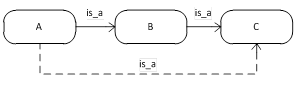
\includegraphics[width=200pt]{isa.png}
	\caption{Relasi \textit{is\_a}}
	\label{fig:is_a}
\end{figure}

Pada GO contoh dari relasi ini di tunjukkan seperti pada Gambar \ref{fig:contoh_is_a}. Terlihat bahwa \textit{single organism cellular process is a single organism process} dan \textit{single organism process is a biological process}, maka dari itu \textit{single organism cellular process is a biological process}.

\begin{figure}[h!] % Gunakan \begin{figure*} untuk memasukkan Gambar
	\centering
	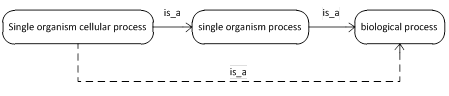
\includegraphics[width=200pt]{contoh_is_a.png}
	\caption{Contoh relasi \textit{is\_a}}
	\label{fig:contoh_is_a}
\end{figure}
\begin{flushleft}
	2. \textit{part\_of}
\end{flushleft}\par
Relasi \textit{part of}  ini menjelaskan bahwa apabila A \textit{part of} B, maka A merupakan salah satu kelas yang ada di dalam B. Relasi ini biasanya dipakai untuk menjelaskan suatu proses yang memiliki beberapa proses di dalamnya. Pada Gambar \ref{fig:part_of} menunjukkan hubungan \textit{part of} antara A dan B, sehingga apabila proses B tidak ada maka proses A pun tidak ada, tetapi apabila A tidak ada belum tentu B tidak ada.
\begin{figure}[h!] % Gunakan \begin{figure*} untuk memasukkan Gambar
	\centering
	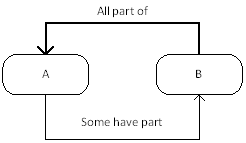
\includegraphics[width=200pt]{part_of.png}
	\caption{Relasi \textit{part\_of}}
	\label{fig:part_of}
\end{figure}
\par
Pada GO contoh relasi ini ditunjukkan seperti pada Gambar \ref{fig:contoh_part_of} yang menunjukkan bahwa \textit{mitochondrial membrane merupakan part of mitochondrion}.
\begin{figure}[h!] % Gunakan \begin{figure*} untuk memasukkan Gambar
	\centering
	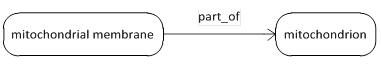
\includegraphics[width=200pt]{contoh_part_of.png}
	\caption{Contoh relasi \textit{part\_of}}
	\label{fig:contoh_part_of}
\end{figure}

\begin{flushleft}
3. \textit{has\_part}
\end{flushleft}\par
Relasi \textit{has part} merupakan kebalikan dari \textit{part of}. Apabila part of menunjukkan dari bagian kecil ke bagian yang lebih besar, maka \textit{has part} menunjukkan bagian besar memiliki bagian-bagian yang lebih kecil. Pada Gambar \ref{fig:has_part} menunjukkan skema relasi \textit{has part}, B memiliki bagian berupa A.
\begin{figure}[h!] % Gunakan \begin{figure*} untuk memasukkan Gambar
	\centering
	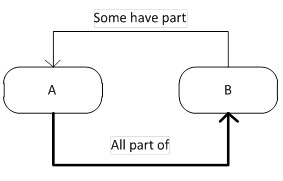
\includegraphics[width=200pt]{has_part.png}
	\caption{Relasi \textit{has\_of}}
	\label{fig:has_part}
\end{figure}
\par
Di dalam GO relasi ini ditunjukkan dengan hubungan antara \textit{nucleus} dengan \textit{chromosome} seperti terlihat pada Gambar \ref{fig:contoh_has_part}.
\begin{figure}[h!] % Gunakan \begin{figure*} untuk memasukkan Gambar
	\centering
	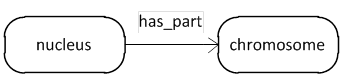
\includegraphics[width=200pt]{contoh_has_part.png}
	\caption{Contoh relasi \textit{has\_of}}
	\label{fig:contoh_has_part}
\end{figure}
\begin{flushleft}
4. \textit{regulates}
\end{flushleft}\par
Relasi \textit{regulates} merupakan relasi yang umum terdapat pada GO. Relasi ini menunjukkan bahwa node yang satu mempengaruhi node yang lain. Pada Gambar \ref{fig:regulates} menunjukkan bahwa B \textit{regulates} A, yang artinya apabila B merupakan suatu proses maka proses yang terjadi pada B akan mempengaruhi proses pada A, tetapi proses B tidak selalu terpengaruh dengan proses A.
\begin{figure}[h!] % Gunakan \begin{figure*} untuk memasukkan Gambar
	\centering
	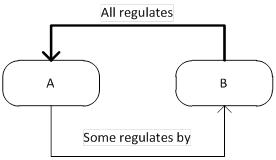
\includegraphics[width=200pt]{regulates.png}
	\caption{Relasi \textit{regulates}}
	\label{fig:regulates}
\end{figure}
\par
Relasi ini pada GO dicontohkan hubungan antara \textit{activation of reciprocal meiotic recombination} mempengaruhi proses dari \textit{meiotic cell cycle} yang ditunjukkan pada Gambar \ref{fig:contoh_regulates}.
\begin{figure}[h!] % Gunakan \begin{figure*} untuk memasukkan Gambar
	\centering
	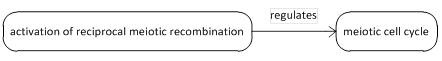
\includegraphics[width=200pt]{contoh_regulates.png}
	\caption{Contoh relasi \textit{regulates}}
	\label{fig:contoh_regulates}
\end{figure}
\begin{flushleft}
\textbf{Model Informasi}
\end{flushleft}
Setelah mendapatkan model ontologi dari GO maka tahap selanjutnya adalah merancang model informasi. Informasi yang akan ditampilkan kepada pengguna sistem adalah informasi yang terdapat pada GO akan ditampilkan dengan cara pengguna memasukkan kata kunci yang akan di cari. Kemudian setelah ditemukan untuk mengetahui lebih lanjut mengenai informasi dari hasil yang ditemukan maka pengguna dapat masuk ke halaman detail dengan menggunakan link yang ada pada hasil tersebut. Tabel \ref{tab:kelas} menunjukkan kelas yang ada di dalam sistem ini.

\begin{table}[h!]
	\footnotesize
	\caption{Kelas pada sistem GO}
	\centering
	\begin{tabulary}{0.47\textwidth}{LLL}
		\toprule
		\parbox{8em}{Kelas}&\parbox{8em}{Atribut} & Proses \\
		\midrule
		SearchForm & Keyword, Ontology & ViewForm()\par submitKeyword(string)\\
		Result & QueryResult &  viewQResult()\par viewOntology()\par viewDetail(string)
		\\
		\bottomrule
	\end{tabulary}
	\label{tab:kelas}
\end{table}

\begin{flushleft}
\textbf{Model User}
\end{flushleft}
Use Case sistem yang akan dibuat dapat dilihat pada Gambar \ref{fig:use_case}.
\begin{figure}[h!] % Gunakan \begin{figure*} untuk memasukkan Gambar
	\centering
	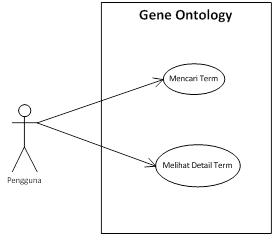
\includegraphics[width=200pt]{use_case.png}
	\caption{\textit{Use case diagram} sistem GO}
	\label{fig:use_case}
\end{figure}
\par
Pada use case ini menunjukkan bahwa pengguna dapat melakukan pencarian \textit{term} berdasarkan kata kunci yang ingin dicari. Kemudian setelah menemukan kata kunci yang dicari pengguna dapat melihat detail dari kata kunci tersebut.

Berdasarkan \textit{use case} pada Gambar \ref{fig:act1} maka dibuat \textit{activity diagram} untuk \textit{use case} mencari \textit{term} dan Gambar \ref{fig:act2} untuk \textit{use case} melihat \textit{detail term}. 

\begin{figure}[h!] % Gunakan \begin{figure*} untuk memasukkan Gambar
	\centering
	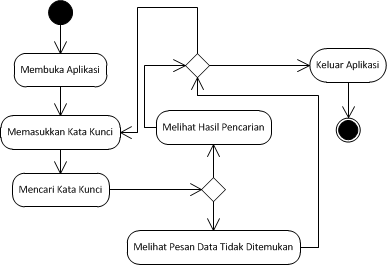
\includegraphics[width=100pt]{act1.png}
	\caption{\textit{Activity diagram} mencari term}
	\label{fig:act1}
\end{figure}

\begin{figure}[h!] % Gunakan \begin{figure*} untuk memasukkan Gambar
	\centering
	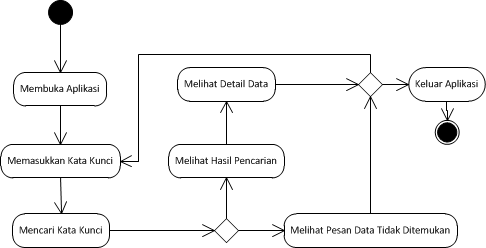
\includegraphics[width=100pt]{act2.png}
	\caption{\textit{Activity diagram} melihat detail term}
	\label{fig:act2}
\end{figure}

Dari \textit{activity diagram} yang dibuat maka dapat dibuat \textit{sequence diagram}. \textit{Sequence diagram} ini menunjukkan langkah detail yang akan dilakukan pengguna pada saat menggunakan sistem ini. Pada Gambar \ref{fig:sequence_1} menunjukkan \textit{sequence diagram} untuk \textit{use case} mencari \textit{term} dan Gambar \ref{fig:sequence_2} \textit{sequence diagram} untuk \textit{use case} melihat detail \textit{term}.
\begin{figure}[h!] % Gunakan \begin{figure*} untuk memasukkan Gambar
	\centering
	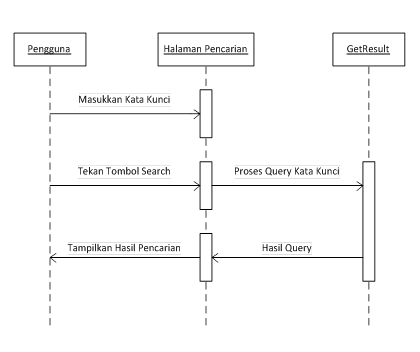
\includegraphics[width=200pt]{sequence_1.png}
	\caption{\textit{Sequence diagram} mencari \textit{term}}
	\label{fig:sequence_1}
\end{figure}
\begin{figure}[h!] % Gunakan \begin{figure*} untuk memasukkan Gambar
	\centering
	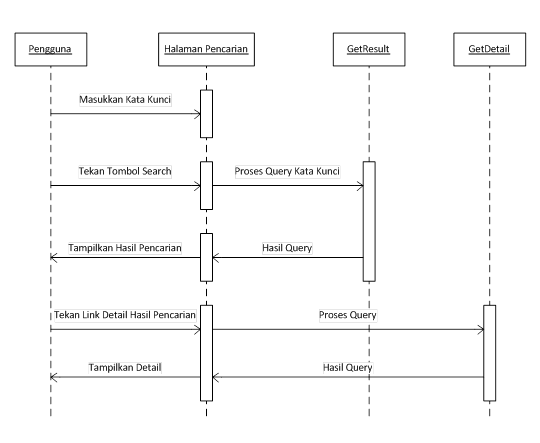
\includegraphics[width=200pt]{sequence_2.png}
	\caption{\textit{Sequence diagram} melihat detail \textit{term}}
	\label{fig:sequence_2}
\end{figure}
\subsection*{Fase Implementasi dan Desain}
\begin{flushleft}
\textbf{Parsing Ontologi}
\end{flushleft}
Ontologi merupakan salah satu cara yang digunakan untuk merepresentasikan pengetahuan. Ontologi menggunakan Uniform Resource Identifier (URI) untuk membentuk struktur dokumennya. URI ini digunakan untuk memberikan keterangan pada suatu objek. Objek dari ontologi terdiri dari tiga bagian yang disebut \textit{triples}. \textit{Triples} ini terdiri dari\textit{ subject}, \textit{predicate} dan \textit{object}. Tujuan dari dilakukan \textit{parsing} ontologi adalah untuk membuat ontologi dapat dibaca dan dipahami oleh pembuat sistem.

Model  data ontologi yang digunakan pada penelitian ini menggunakan RDF. RDF berisi kumpulan kumpulan \textit{triples} yang disimpan dalam format XML. Model data ini dipilih karena merupaka model data yang menjadi standar pada ontolgi, sehingga terdapat banyak \textit{parser} yang dapat melakukan parsing terhadap data RDF.

Parser yang digunakan pada penelitian ini adalah RDFLib. RDFLib merupakan package dari bahasa pemrograman python yang dapat melakukan \textit{parsing} terhadap data ontologi.  RDFLib dipilih karena memiliki beberapa kelebihan, seperti dapat mem-parsing berbagai jenis model data, dapat menyimpan graph dari suatu ontologi, dapat menyimpan data pada \textit{memory} maupun secara presistent, dan dapat menggunakan SPARQL untuk melakukan operasi pada data ontologi.

Untuk penggunaan RDFLib pada python maka sistem harus memanggil package RDFLib tersebut dengan syntax seperti pada Gambar \ref{fig:import}.

\begin{figure}[h!] % Gunakan \begin{figure*} untuk memasukkan Gambar
	\centering
	
\includegraphics[width=100pt]{import.png}
	\caption{Pemanggilan \textit{package} RDFLib}
	\label{fig:import}
\end{figure}

Untuk melakukan parsing terhadap data ontologi maka syntax yang diperlukan seperti pada Gambar \ref{fig:parsing}. Pada Gambar \ref{fig:parsing} terlihat bahwa RDFLib melakukan parsing terhadap data ontology GO.

\begin{figure}[h!] % Gunakan \begin{figure*} untuk memasukkan Gambar
	\centering
	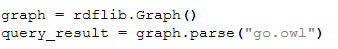
\includegraphics[width=200pt]{parsing.png}
	\caption{Proses \textit{parsing} ontologi}
	\label{fig:parsing}
\end{figure}

\begin{flushleft}
	\textbf{Implementasi Model Informasi}
\end{flushleft}

Pada proses implementasi model informasi maka dibuat \textit{user interface} yang akan digunakan oleh pengguna. Penelitian ini akan menghasilkan sistem yang berbasis web dengan menggunakan \textit{web framework} Flask yang merupakan \textit{web framework} python yang ringan. Pembuatan halaman web menggunakan HTML. Dengan dibuat sistem yang berbasis web maka sistem ini dapat dibuka di komputer manapun tanpa melakukan proses instalasi. Halaman yang dibuat pada sistem ini ditunjukkan pada Tabel \ref{tab:info}.

\begin{table}[h!]
	\footnotesize
	\caption{Halaman yang dibuat pada sistem GO}
	\centering
	\begin{tabulary}{0.47\textwidth}{LL}
		\toprule
		\parbox{8em}{Halaman} & URL \\
		\midrule
		Search & url/index\\
		Result & url/result\\
		Detail & url/detail\\
		\bottomrule
	\end{tabulary}
	\label{tab:info}
\end{table}

Gambar \ref{fig:search} merupakan halaman Search yang digunakan pengguna untuk melakukan pencarian terhadap kata kunci yang ingin dicari.

\begin{figure}[h!] % Gunakan \begin{figure*} untuk memasukkan Gambar
	\centering
	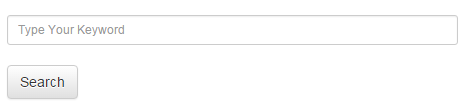
\includegraphics[width=200pt]{search.png}
	\caption{Halaman \textit{search}}
	\label{fig:search}
\end{figure}

\begin{flushleft}
	\textbf{Implementasi Model User}
\end{flushleft}

Pengguna akan menuliskan kata kunci pada search form yang sudah disediakan. Kemudian apabila tombol Search ditekan maka sistem akan melakukan pencarian terhadap kata kunci yang diberikan. Proses pencarian tersebut dilakukan pada data GO dengan menggunakan SPARQL seperti tampak pada Gambar \ref{fig:sparql}.

\begin{figure}[h!] % Gunakan \begin{figure*} untuk memasukkan Gambar
	\centering
	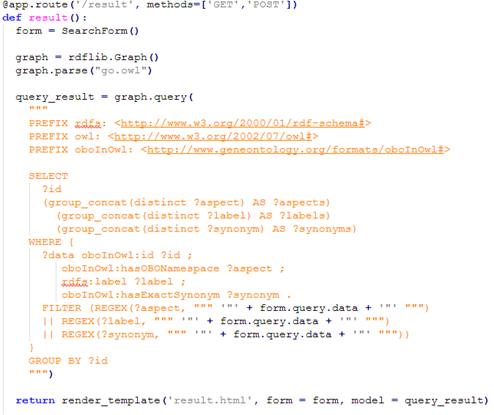
\includegraphics[width=200pt]{sparql.png}
	\caption{\textit{Syntax} proses pencarian \textit{term}}
	\label{fig:sparql}
\end{figure}

Pada Gambar \ref{fig:sparql} terdapat syntax SPARQL, dengan struktur PREFIX dan perintah SELECT. PREFIX digunakan untuk mempersingkat URI yang digunakan pada perintah SELECT. Pada perintah SELECT terdapat bagian yang akan ditampilkan pada halaman web yaitu \textit{?id}, \textit{?aspects}, \textit{?labels} dan \textit{?synonyms}. Kemudian terdapat bagian WHERE menunjukkan variabel apa saja yang akan diambil dari data ontologi. Pada bagian WHERE ini merupakan \textit{triple} yang berupa \textit{subject}, \textit{predicate} dan \textit{object}. \textit{Subject} pada query ini disimbolkan dengan ?data. \textit{Predicate} berupa URI dan atribut yang akan diambil, URI diganti dengan PREFIX agar lebih ringkas dalam penulisannya sebagai contoh oboInOwl:id. \textit{Object} digunakan untuk menyimpan data yang didapat dari hasil query, sebagai contoh \textit{object} ?id. Gambar \ref{fig:result} merupakan hasil dari query yang ditampikan pada halaman result.

\begin{figure}[h!] % Gunakan \begin{figure*} untuk memasukkan Gambar
	\centering
	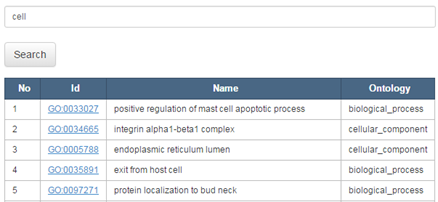
\includegraphics[width=200pt]{result.png}
	\caption{Halaman hasil pencarian \textit{term}}
	\label{fig:result}
\end{figure}


%----------------------------------------------------------------------------------------
%	BAGIAN KESIMPULAN
%----------------------------------------------------------------------------------------

%----------------------------------------------------------------------------------------
%	KESIMPULAN DAN SARAN
%----------------------------------------------------------------------------------------

%----------------------------------------------------------------------------------------
%	BAGIAN DAFTAR PUSTAKA
%----------------------------------------------------------------------------------------

\renewcommand{\refname}{DAFTAR PUSTAKA}
\nocite{*}
\printbibliography

%----------------------------------------------------------------------------------------

\end{document}